\chapter{The Kalman Filter}

In order to design a optimal controller for the quad-rotor a State-Estimator is required. The reason for this is simple: one doesn't have access to all the system states. For example one can't measure the angle velocity of the propellers as the Quad-rotor doesn't have a hall sensor. Due to the use of inexpensive sensors a  stochastic filter or full non-linear model of the sensors had to be developed. Thus, the Kalman Filter was chosen as it is a ideal filter and is capable of estimating angle and rate of change of angle with great accuracy.  \cite{acclerometer_bais}.

\begin{figure}[h]
	\centering
	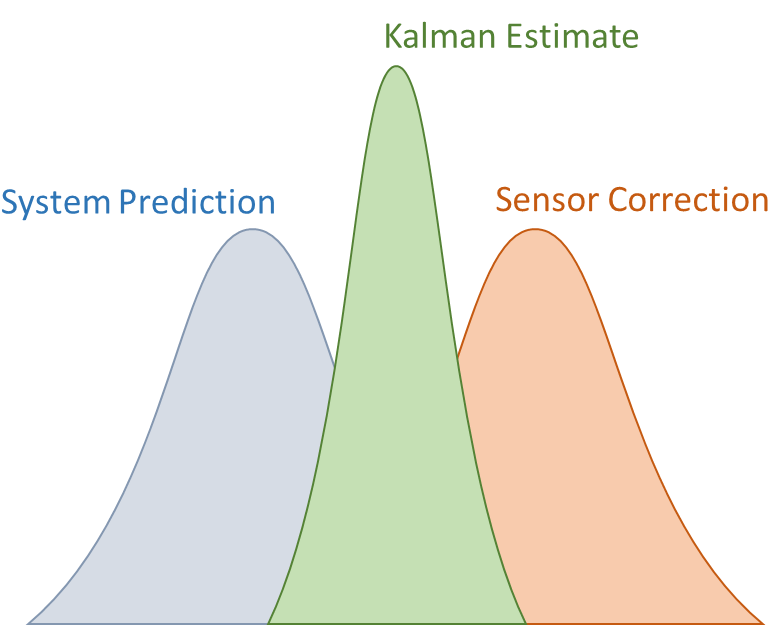
\includegraphics[width =0.4\paperwidth]{\DocRoot/images/kalman_gauss}
	\caption{Gaussian representation of the Kalman Filter}
	\label{Fig: Kalman Filter gauss}
\end{figure}

When a Kalman Filter is being implemented the noise present in the system and senors has to be to Gaussian zero-mean, which is usually denoted as \gls{noiseinsysystem} and \gls{noiseinoutput} respectively. If this criteria is met the filter will yield a new linear system model which is free of noise. The Filter works by adding a prediction produced by the plant model from known inputs, and a correction from the data measured by sensors. This process can be best visualized by figure \ref{Fig: Kalman Filter gauss}, where the plant estimate and the sensor estimate have been fused together to achieve a best guess of the actual state. The Kalman Filter is similar to the Luenberger Observer \footnote{An Observer is used to estimate unmeasurable states by means of a system model and some measurable outputs.}, but the observer gains are chosen in an optimal manner. The Kalman Gain \gls{kalmangain} defines by how much the model estimate has to be corrected by the sensor measurements. Hence, if the noise in the sensors is greater than the noise in the model the senor measurements are trusted more to estimate the required states, and thus assigned a greater weighting. If the noise present in the system states is greater than the noise present in the sensor, then sensor readings will be trusted more to estimate the required states. Thus, in short, the Kalman Filter is a state observer for the stochastic case. In order to apply this filter one must define the system in a discrete liner state space form.

\begin{equation}\label{eq:descrete_state_space_model}
\begin{split}
\underline{x}_{k+1} &= \gls{Transitionmatrix} \underline{x}_k + \gls{Bmatrix}_d\underline{u}_k + \gls{couplingmatrix}\underline{w}_k \\
\underline{z}_{k}      &= \gls{Cmatrix}_d \underline{x}_k + \underline{v}_k
\end{split}
\end{equation}


The filter , whose linear model is described in \ref{eq:descrete_state_space_model}, can be seen as a \gls{lti}  system operating in parallel to the real physical system in order to generate an optimal estimate  $\underline{\hat{x}}$ of all states whereas compensating for the noise in the plant \footnote{Note superscript $d$ notation is dropped for simplicity, E.g ($\gls{Bmatrix} _d~=~ \gls{Bmatrix} $).}. The filter removes/reduces the noise present in the plant by minimizing the error covariance matrix of the estimated states. The covariance matrix is commonly denoted as follows:- 

\begin{equation}
\gls{covariancematrix}= E[\tilde{\underline{x}_k}~{\tilde{\underline{x}_k}}^\top]
\end{equation}
where ${\tilde{\underline{x}}}_k$ is the error in the estimated states.

Note an expression for the \gls{covariancematrix} matrix must be developed from the initial system to begin the filter derivation. Therefore from \eqref{eq:descrete_state_space_model}, the best state estimate can be achieved :-

\[\hat{\underline{x}}_{k+1|k}  =\gls{Transitionmatrix}_k\hat{\underline{x}}_{k|k} + \gls{Bmatrix}{\underline{u}}_k\]


\section{Development of the Kalman Filter}
As seen from figure \ref{fig:Kalman Filter flow diagram} the Kalman Filter is made up of two stages, a predict stage and a correct stage. The predict stage generates an estimate of the required states by means of an ideal system model whose inputs are known. After the estimate is found then the covariance error is measured (this is the aspect to minimize). The covariance error indicates by how much the state estimates differ from the ideal signal. After this the correct stage begins and the Kalman gain \gls{kalmangain} is calculated by means of the covariance error and the covariance of  the sensor data. Next, the initial estimate is corrected by means of sensor data which is scaled appropriately by the Kalman gain \gls{kalmangain}. Finally the covariance error is corrected by means of the Kalman gain \gls{kalmangain} and after which the Kalman starts, hence the recursive aspect of the Kalman Filter.  			


Thus, implement the Kalman filter a recursive algorithm  needs to developed. In order to accomplish this assume access to the previous estimate $\hat{x}_{k|k}$, as the initial value $\hat{x}_{0|0}$ it is possible to define a recursive. If the previous estimate is known any future value can be calculated, but this can only be done if the noise signal is zero mean that is, E[$w_k$] = E[$v_k$] = 0 . Hence, the best estimate can be derived from \eqref{eq:descrete_state_space_model} by taking the mean value of $\underline{w}_k$, doing so will yield the following:-

\begin{equation}
\hat{\underline{x}}_{k+1|k} =\gls{Transitionmatrix}_k\hat{\underline{x}}_{k|k} + \gls{Bmatrix} {\underline{u}}_k
\label{eq: best estimate equation latex}
\end{equation}
Therefore the one-step-ahead  \textit{Predictive measurement} can be defined as follows:-
\begin{equation*}
\hat{z}_{k+1} = \gls{Cmatrix}\hat{x}_{k+1|k}
\end{equation*}

At time (k+1) , one can measure $\gls{measurement}_{+1}$ from the plant, thus define the \textit{Predict error} $\tilde{z}$ as follows:-
\begin{equation}
\tilde{\underline{z}}_{k+1} = {\underline{z}}_{k+1 }- \hat{\underline{z}}_{k+1}
\label{eq: prediction error}
\end{equation}

Thus, to improve the state estimate one can add some proportion of the prediction error \eqref{eq: prediction error} to each element of the state vector to drive the prediction error to zero as follows:-
\begin{equation}
\hat{\underline{x}}_{k+1|k+1}  = \gls{Transitionmatrix}\hat{\underline{x}}_{k|k} +\gls{Bmatrix} {\underline{u}}_k+ \gls{kalmangain}\tilde{\underline{z}}_k
\label{eq: error corrected equation}
\end{equation}

Knowing \eqref {eq: best estimate equation latex},  \eqref{eq: prediction error} and \eqref{eq: error corrected equation} and filling in one gets the following equation:-
\begin{equation}
\hat{\underline{x}}_{k+1|k+1} = \gls{Transitionmatrix}\hat{\underline{x}}_{k|k} +\gls{Bmatrix}{\underline{u}}_{k} + \gls{kalmangain} [{\underline{z}}_{k+1} - { C}(\gls{Transitionmatrix} \hat{\underline{x}}_{k|k} + \gls{Bmatrix}{\underline{u} }_k) ] \label{eq : kalman gain from art of control long}
\end{equation}

Thus matrix/variables are grouped together for ease of computation and yields the following:- 
\begin{equation}
\hat{\underline{x}}_{k+1|k+1} = [{I -\gls{kalmangain}\gls{Cmatrix}}][\gls{Transitionmatrix} \hat{\underline{x}}_{k|k} +\gls{Bmatrix} {\underline{u}}_k] + \gls{kalmangain}z_{k+1} \label{eq: kalman equation from art of controll}
\end{equation}

Equation \ref{eq: kalman equation from art of controll} can be written as follows.
\begin{equation}
\hat{\underline{x}}_{k+1|k+1} = { F}\hat{\underline{x}}_{k|k} + { H}{\underline{u}}_k + \gls{kalmangain}{z}_{k+1} \label{Eq: Kalman Equation Representation used in our reporty}
\end{equation}
Where in \eqref{Eq: Kalman Equation Representation used in our reporty} ${ F} =  [{I -\gls{kalmangain} \gls{Cmatrix} }]\gls{Transitionmatrix}$; $H =  [{I -\gls{kalmangain} \gls{Cmatrix} }] \gls{Bmatrix} $. Thus each matrix is made up of a mix of prediction and correction values.

It was assumed in this project that the separate noise signals were independent of each other, thus allowing \gls{noisecomatrix} and \gls{noisecoplantmatrix} to be covariance matrices. A large value for \gls{noisecomatrix} implies a lot of noise is present in the measurement data and thus more emphasis is placed in the predictions. A large value of \gls{noisecoplantmatrix} implies that there is more noise in the states than in the measurement data and thus the measurement data is followed more closely. As \gls{covariancematrix} is to be minimized, an expression for the estimation of the covariance error can be obtained as follows (\enquote{Predict} stage):-

\begin{equation}
\gls{covariancematrix}^* = \gls{Transitionmatrix}\gls{covariancematrix}_{-1}\gls{Transitionmatrix}^{\intercal} + \gls{couplingmatrix}\gls{noisecoplantmatrix}\gls{couplingmatrix}^{\intercal} \label{eq: P equation for the kalman filter}
\end{equation}

Thus the Kalman gain \gls{kalmangain} can be defined as follows. Note the Kalman Gain \gls{kalmangain} must be updated at each iteration to correct the measurement data so as to obtain an optimal estimate of the required states. The equation governing this update process is as follows (\enquote{Correct} stage) :-

\begin{equation}
\gls{kalmangain}_{k} = \gls{covariancematrix}^*\gls{Cmatrix}^{\intercal}(\gls{Cmatrix}\gls{covariancematrix}^*\gls{Cmatrix}^{\intercal} + \gls{noisecomatrix})^{-1}
\end{equation} 

Finally the covariance error can be corrected as follows:-
\begin{equation}
\gls{covariancematrix} = (I - \gls{kalmangain}_k\gls{Cmatrix})\gls{covariancematrix}^{*}
\end{equation}


From \eqref{eq: P equation for the kalman filter} the performance of this filter depends heavily upon the accuracy of \gls{noisecoplantmatrix} and \gls{noisecomatrix}. Note \gls{noisecomatrix} can often be intelligently estimated from knowledge of the system under control. The derivation of \gls{noisecoplantmatrix} is  a problem as often very little real information will be known about the noise present in the states.  Therefore \gls{noisecoplantmatrix} is often guessed and \gls{noisecomatrix} and \gls{noisecoplantmatrix} are tuned together to get an adequate result for the control of the device.
\begin{comment}
	\tikzset{%
	block/.style    = {draw, thick, rectangle, minimum height = 3em,minimum width = 3em},
	
	input/.style    = {coordinate}, % Input
	
	output/.style   = {coordinate} % Output

	block/.style    = {draw, thick, rectangle, minimum height = 3em,minimum width = 3em},

	gain/.style     = {draw, thick, isosceles triangle, minimum height = 2em,isosceles triangle apex angle=60},

	port/.style     = {inner sep=0pt, font=\tiny},
	
	sum/.style n args = {4}{draw, circle, node distance = 2cm, minimum size=5mm, alias=sum,
		append after command={
			node at (sum.north) [port, below=1pt] {$#1$}
			node at (sum.west) [port, right=1pt] {$#2$}
			node at (sum.south) [port, above=1pt] {$#3$}
			node at (sum.east) [port, left=1pt] {$#4$}
		},
	}, % Adder
	
	joint/.style    = {circle, draw, fill, inner sep=0pt, minimum size=2pt},
	
}
% Defining string as labels of certain blocks.
\newcommand{\suma}{\Large$+$}
\newcommand{\inte}{$\displaystyle \int$}
\newcommand{\derv}{\huge$\frac{d}{dt}$}
\end{comment}

\subsection{Kalman Filter Operation}

As described in the previous sections, the Kalman Filter extracts state estimates from noisy signals. This can be done by obtaining statistical information of the noise present in both the plant and the measurement data, knowing this the filter can optimally estimate the state of interest. This information is given in form of the plant and measurement noise covariances, \gls{noisecomatrix} and \gls{noisecoplantmatrix}. The algorithm that the filter performs can be described as follows:


First, the \gls{noisecoplantmatrix} and \gls{noisecomatrix} covariance matrices are calculated through trial and error. An initial state estimate $\hat{\underline{x}}_{0|0}$ and its error covariance $\text{\bf P}_0$ are entered. The Kalman Gain matrix, \gls{kalmangain} is computed based on \text{\bf P}, \gls{noisecomatrix} and the transition matrix \gls{Transitionmatrix}. The estimate is then updated with the current measurement data and after which a new error covariance computed. The algorithm then starts again from the beginning. The output from the filter is an estimate of the states and the error covariance matrix, {\bf P}. Figure \ref{fig:Kalman Filter flow diagram}, shown below is a flow diagram of the Kalman Filter algorithm.   


		\begin{figure}[h]
			\renewcommand{\baselinestretch}{1.5} 	
			\centering
			\resizebox{14cm}{8cm}{\begin{tikzpicture}[auto, thick, node distance=2cm, >=triangle 45]
			
			%
			% Styles for states, and state edges
			%
			\tikzstyle{state} = [{rectangle, rounded corners, draw=black, very thick, text width=20.0em, minimum height=4em, text centered}]
			\tikzstyle{stateEdgePortion} = [black,thick];
			\tikzstyle{stateEdge} = [stateEdgePortion,->];
			\tikzstyle{edgeLabel} = [pos=0.5, text centered, font={\sffamily\small}];
			
			
			%
			% Position States
			%
			\node[state, name=predict] {{{\LARGE}{\bf Model Update} (\enquote{Predict})}   \\ 
				{   (1) Predict State  \\  \vspace{-0.25cm}
					\hh $\hat{x}^{*}_{k} = \gls{Transitionmatrix}\hat{x}_{k-1} + \gls{Bmatrix}u_{k}$\\ 
					(2) Predict Error Covariance \\ \vspace{-0.25cm}
					\hh $\gls{covariancematrix}^* = \gls{Transitionmatrix}\gls{covariancematrix}_{-1}\gls{Transitionmatrix}^{\intercal} + \gls{noisecoplantmatrix}$}};
			
			
			\node[state, name=correct, right of=predict, xshift=20em] {{\bf Measurement Update} (\enquote{Correct}) \\ 
				{   (1) Compute Kalman Gain\\  \vspace{-0.25cm}
					\hh $\gls{kalmangain}_{k} = \gls{covariancematrix}^*\gls{Cmatrix}^{\intercal}(\gls{Cmatrix}\gls{covariancematrix}^*\gls{Cmatrix}^{\intercal} + \gls{noisecomatrix})^{-1}$\\ 
					(2) Update Estimate with Measurement $\gls{measurement}$ \\ \vspace{-0.25cm}
					\hh $\hat{x}_k = \hat{x}^{*}_k + \gls{kalmangain}_k(z_k - \gls{Cmatrix}\hat{x}_k^{*})$\\
					(3) Update Error Covariance  \\ \vspace{-0.25cm}
					\hh $\gls{covariancematrix} = (I - \gls{kalmangain}_k\gls{Cmatrix})\gls{covariancematrix}^{*}$
					
				}};
				
				
				%
				% Connect States via edges
				%
				\draw (predict.north) 
				edge[stateEdge, bend left=45] node[edgeLabel, xshift=-3em]{} 
				(correct.north); 
				
				\draw ($(predict.west) + (0,2.5em)$) 
				edge[stateEdgePortion] node[edgeLabel, yshift=+2.1cm]{} 
				($(predict.east) + (0,2.5em)$); 
				
				\draw (correct.south) 
				edge[stateEdge, bend left=45] node[edgeLabel, xshift=-3em]{} 
				(predict.south); 
				
				\draw ($(correct.west) + (0,4.0em)$) 
				edge[stateEdgePortion] node[edgeLabel, yshift=+2.1cm]{} 
				($(correct.east) + (0,4.0em)$); 
				
				
				
				% 
				% inital states to start the filter
				%
				\node[ name=inital, below of=predict, left of=predict, xshift = -0.68em ,yshift=-8em]{Initial Estimates for $\hat{x}_{k-1}$ and $\gls{covariancematrix}_{-1}$};
				
				\draw ($(inital.north) + (0,0)$) 
				edge[stateEdge] node[edgeLabel, yshift=+2.1cm]{} 
				($(predict.south) + (-5.4em,0)$); 
				\end{tikzpicture}}
					\caption{Kalman Filter flow diagram}
					\label{fig:Kalman Filter flow diagram}
			\end{figure}




\section{Kalman Filter Used in Project}
 There were three Kalman filters developed for this report; a steady state Kalman Filter whose Kalman Gains remains constant over time, a Kinematic Kalman Filter which is based on the Kalman filter presented in Ersson and Hu \cite{ersson2001state} and an Extended Kalman Filter. Note all Kalman Filters investigated in this project will be developed in this section, while the implementation and tuning will be presented in Chapter \ref{chap: kalman implem}

\subsection{The Static Kalman Filter}
The Static Kalman Filter, which will be developed in the this sections uses a constant \gls{kalmangain} which is found by means of the Kalman Filter Algorithm presented in \ref{fig:Kalman Filter flow diagram}. In practice, the time-varying Kalman gain \gls{kalmangain} tends towards a steady value \cite{LQG_mit}. Hence, when the Kalman Filter is used on the quad-rotor the Kalman Gain \gls{kalmangain} will converge to a constant value, thus, a constant Kalman Gain \gls{kalmangain} can be used to estimate the required states. As the Static Kalman Filter uses a constant \gls{kalmangain} term, the observer produced by this method is a optimal Luenberger Observer\footnote{This Static Kalman Gain can be found by using the \textit{lqg} commend in MatLab}. The model used in the Kalman Filter for the pitch, roll and yaw axes are the same ones developed in \eqref{eq: pitch model}, \eqref{eq: roll model} and \eqref{d2ydt2}. Note as these are continuous equations, a mapping of the continuous time model to a discrete model has to take place which was done by means of the Matrix Exponential. After the discrete Static Kalman Filter was developed the \gls{kalmangain} terms shown in \eqref{eq: static kalman equations for micro} was adjusted by methods presented in Chapter \ref{chap: kalman implem} until an optimal response was achieved. 
\subsection{Derivation of state space equations}
As the Kalman Filter is required run on a micro-controller, the Kalman Filter expressed in  \ref{Eq: Kalman Equation Representation used in our reporty} has to be expressed in its most compact format so as to reduce computational effort and improve its accessibility. These requirement lead to the following definition for the Static Kalman Filter:-
%{Eq: Kalman Equation Representation used in our reporty}
\begin{equation}
\begin{bmatrix}																
\hat{x}_1		         			\\
\hat{ x}_2		
\end{bmatrix}_{k+1}
=
\begin{bmatrix}
F_{11}	& F_{12 } \\
F_{21}	& F_{22}
\end{bmatrix}
\begin{bmatrix}											
\hat{ x}_1		         			\\
\hat{ x}_2		
\end{bmatrix}_{k}	
+
\begin{bmatrix}
H_1 \\
H_2
\end{bmatrix}
{ u}_k
+
\begin{bmatrix}
K_{11}	& K_{12 } \\
K_{21}	& K_{22}
\end{bmatrix}
\begin{bmatrix}											
{ z}_1		         			\\
{z}_2		
\end{bmatrix}_{k+1}	
\label{eq: static kalman equations for micro}
\end{equation}

For the quad-rotor the state ${ x_1}$ is angular velocity ${\bf \alpha}$ and the state ${ x_2}$ is angular acceleration $\dot{\bf \alpha}$  


\subsection{The Kinematic Kalman Filter}
Unlike the Kalman Filter presented in the previous section, the Kalman filter being developed in the following section uses a pure kinematic relationship, thus a model of the plant is not required. This kinematic relationship uses the current gyroscope data to relate the derivative of the rotation matrix to the rotation matrix and is defined as follows:-

\begin{equation}
\dot{\gls{rotationmatrix}} =  \underbrace{\left[\begin{array}{ccc} 0 & \gls{wz} & -\gls{wy}\\ -\gls{wz} & 0 & \gls{wx}\\ \gls{wy}&-\gls{wx} & 0 \end{array}\right] }_{\text{\gls{skewmatrix}}}\gls{rotationmatrix}  \label{eq: rotation matrix related using the gyro readings}
\end{equation} 




\begin{description}[itemsep=0.5mm]
	\item[{\bf Where:-}]
	\item[\gls{skewmatrix}:] is a skewed matrix that contains the set of all proper orthogonal matrices and is defined as {$\gls{skewmatrix} \bf= R|R\varepsilon R^{3x3},R^\intercal R = RR^\intercal = I$}
	\item[\gls{wx}, \gls{wy}, \gls{wz}:] are the roll,pitch and yaw angular rates, respectively.
\end{description}

These rates are measured using the gyroscopes onboard the quad-rotor, in the \gls{imu}.

Using \eqref{eq: rotation matrix related using the gyro readings}, the following continuous state space equations presented in \eqref{eq:state space adative kalman equations1} can be used to  represent the system:-
 


\begin{align}
\begin{split}
\dot{\underline{x}} &= \gls{skewmatrix}\underline{x}\\
\underline{y}              &= \underline{x}
\end{split}
\label{eq:state space adative kalman equations1}
\end{align}

However, \eqref{eq:state space adative kalman equations1} is a continuous state space equation. This must be converted to the discrete version since the Kalman Filter must be implemented in discrete form, which is achieved as follows:-

\begin{align}
\begin{split}
\underline{x}_k &= \gls{Transitionmatrix}_k x_{k-1}\\
\underline{y}_k              &= \underline{x}_k
\end{split}
\end{align}



The transformation from the continuous to discrete form is shown in appendix \ref{chap: Rotation Matrix reation}. $\gls{Transitionmatrix}_k$ = $e^{\gls{skewmatrix}\gls{ts}}$, where \gls{ts} is the sampling time of the system. Since \gls{rotationmatrix} is a rotation matrix, and $\underline{x}$ is a column of \gls{Transitionmatrix} (for reasons defined in Section \ref{sec: acc model}). In this filter the dynamic component of the accelerometer measurement is considered to be a disturbance and is assumed to be Gaussian. It is therefore treated as noise and must be removed so as to acquire an accurate estimate. After the noise has been removed from the accelerometer output \eqref{Eq: angles from acc1} can be used to estimate the attitude of the quad-rotor.



\begin{figure}[h]
	\centering
	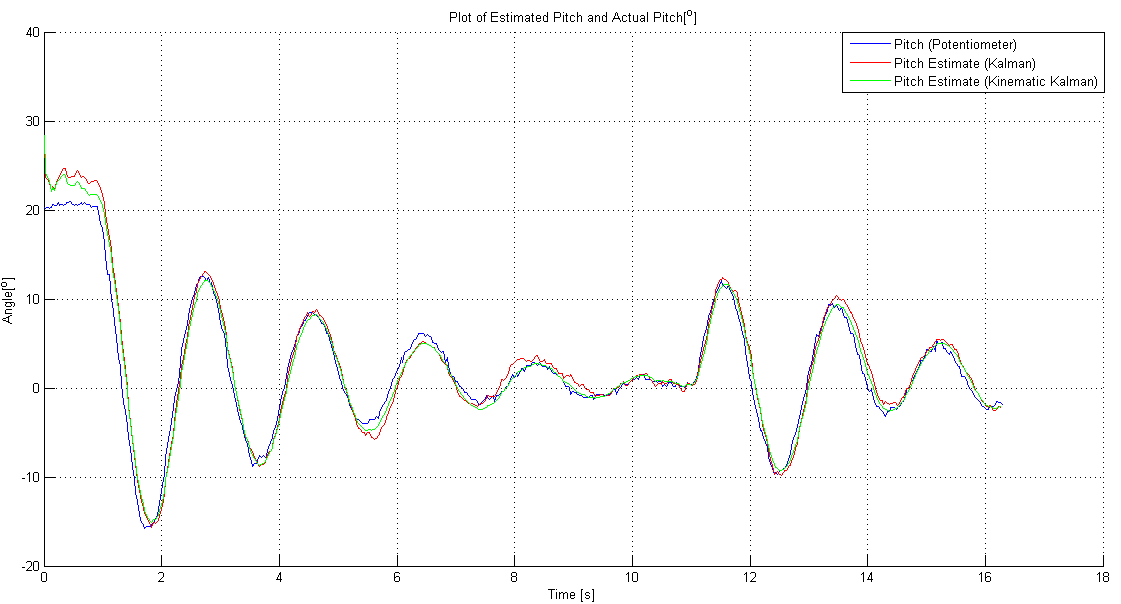
\includegraphics[width =0.7\paperwidth]{\DocRoot/images/kalman_filter_comparsion}
	\caption{Plot of Kalman Filter Estimate, Kinematic Kalman Filter Estimate and Actual Angle of the device}
	\label{Fig: Kalman Filter Estimate and Kinematic Kalman Filter Estimate1}
\end{figure}




\subsection{The Extended Kalman Filter }
As the gyroscope measurement function $h(x_k,\gls{noiseinoutput}_k)$ is highly non-linear it was decided that it was worth while looking at a more advanced Kalman Filter which is capable of dealing with non-linear systems: thus the Extended Kalman Filter was explored (see section \ref{sec: gyroscope sec} for more details on the gyroscope measurement function). Also, as a \gls{gps} module is required to implement positional controller on the quad-rotor it was the natural choice to investigate the \gls{ekf} as it is the de-facto filter used in such systems \cite{An_Introduction_to_the_Kalman_Filter}. 






As the \gls{ekf} filters non-linear functions by means of linearizion of the system around the current
estimate, a method of finding the partial derivatives of both the process and measurement functions is required. Hence, if the process is governed by the \textit{non-linear} stochastic difference equation:-
\begin{equation}
x_k = f(x_{k-1},u_k,\gls{noiseinsysystem}_{k-1})
\end{equation}
and the measurement model by the following stochastic difference equation:-
\begin{equation}
z_k = h(x_k,\gls{noiseinoutput}_k)
\end{equation}

where the random variables \gls{noiseinsysystem} and \gls{noiseinoutput} again represent the process and measurement
noise.



In practice individual values of the individual \gls{noiseinsysystem} and \gls{noiseinoutput}change at each time step. However, one can approximate the state and measurement  without
them as follows:-

\begin{equation}
x_k^* = f(\hat{x}_{k-1},u_k,0) \label{eq: ekf approximate the state}
\end{equation}
Next the measurement model  can be defined by means of the following stochastic difference equation:-
\begin{equation}
z_k = h(x_k^*,0)  \label{eq: ekf approximate the measurement}
\end{equation}

It is important to note that a fundamental flaw of the \gls{ekf} is that the distributions of the various random variables are no longer normal
after undergoing their respective non-linear transformations. The \gls{ekf} is simply an ad-hoc estimator. The \gls{ekf} only approximates the optimality of Bayes’ rule by linearization.


Equation \eqref{eq: ekf approximate the state} is linearized around the control input $u_k$ and the previous estimate using \eqref{eq: jacobain of fx} and the measurement function \eqref{eq: ekf approximate the measurement} is linearized around the $x_k^*$  using  \eqref{eq: jacobain of hx}
\begin{equation}
A_k=\left.\left[\begin{array}{cccc}
\frac{\partial f_{1}}{\partial x_1} &\frac{\partial f_{1}}{\partial x_2} &\dots& \frac{\partial f_{1}}{\partial x_n}\\
\frac{\partial f_{2}}{\partial x_1} &\frac{\partial f_{2}}{\partial x_2} &\dots& \frac{\partial f_{2}}{\partial x_n}\\
\vdots& \vdots& \ddots &\vdots\\
\frac{\partial f_{n}}{\partial x_1} &\frac{\partial f_{n}}{\partial x_2} &\dots&\frac{\partial f_{n}}{\partial x_n} \\
\end{array}\right]\right|_{\hat{x}_k,u_k} \label{eq: jacobain of fx}
\end{equation}

\begin{equation}
C_k=\left.\left[\begin{array}{cccc}
\frac{\partial h_{1}}{\partial x_1} &\frac{\partial h_{1}}{\partial x_2} &\dots& \frac{\partial h_{1}}{\partial x_n}\\
\frac{\partial h_{2}}{\partial x_1} &\frac{\partial h_{2}}{\partial x_2} &\dots& \frac{\partial h_{2}}{\partial x_n}\\
\vdots& \vdots& \ddots &\vdots\\
\frac{\partial h_{n}}{\partial x_1} &\frac{\partial h_{n}}{\partial x_2} &\dots&\frac{\partial h_{n}}{\partial x_n} \\
\end{array}\right]\right|_{\hat{x}_k^*} \label{eq: jacobain of hx}
\end{equation}

Note the above Jacobian can be approximated at each stage on a micro-controller by using the Cauchy’s integral
formula which is defined as follows\cite{Jacobain_approx_paper}:-


\begin{equation}
f^{(n)}(z) = \frac{n!}{2\pi i}\oint_\gamma \frac{f(\kappa)}{(\kappa - z)^{n+1}}d\kappa \label{eq: Cauchy's intrgral formula}
\end{equation}
To implement \eqref{eq: Cauchy's intrgral formula} on a micro-controller it must be approximated as follows:-

\begin{equation}
f^{(n)}(z) \approx \frac{n!}{mh} \sum_{j=0}^{m-1}\frac{f(z+h e^{i\frac{2 \pi j}{m}})}{e^{i\frac{2 \pi j n}{m}}}
\end{equation}

The derivation of a complex-step derivative (first partial derivative) approximation is done by an approximation of a non-linear function with a complex variable using the Taylor's series expansion.

\begin{equation}
f(x+ih) = f(x) + ihf^{'} (x) - h^2\frac{f^{''}(x)}{2!}- ih^3\frac{f^{'''}(x)}{3!}+h^4\frac{f^{4}(x)}{4!} + \dots
\end{equation}
Now taking only the imaginary parts of both sides gives

\begin{equation}
\mathrm{Im}[f(x+ih)] = hf^{'}(x) - h^3\frac{f^{'''}(x)}{3!}+\dots \label{eq: imaginary parts of  Cauchys integral approx}
\end{equation}
Dividing by $h$, rearranging and assuming terms higher than $h^2$ can be ignored since the interval $h$ can be chosen up to the precision of the machine (smallest number the machine can produce) and thus \eqref{eq: imaginary parts of  Cauchys integral approx} can be approximated as follows:-
\begin{equation}
f^{'}(x) = \mathrm{Im}[f(x+ih)]/h \label{eq: how to do differenation on a controller}
\end{equation}
As \eqref{eq: how to do differenation on a controller} is not a function of differences it is more accurate than standard finite difference and more importantly partial derivative can be calculated on a micro-controller using \eqref{eq: how to do differenation on a controller}. 

As a method of approximating the Jacobian matrix has been presented in \eqref{eq: how to do differenation on a controller}, it is now possible to implement the \gls{ekf} on a micro-controller. As the computational capabilities of the micro-controller used in this project were insufficient of implementing an \gls{ekf} it was decided to only simulate the filter. The \gls{ekf} was implemented in MatLab using the algorithm presented in figure \ref{fig: Extended Kalman Filter flow diagram}, and the filtered results can be seen in Figure \ref{Fig:Cross-Correlation of estimated pitch error1}. As can be seen from Figure \ref{Fig:Cross-Correlation of estimated pitch error1} produces the best estimate of the attitude of the quad-rotor; this means an \gls{ekf} would be the ideal filter for both attitude estimation of the quad-rotor as well as \gls{gps} position estimation of the quad-rotor. 


\begin{figure}[h]
	\renewcommand{\baselinestretch}{1.5} 	
	\centering
	\resizebox{16cm}{10cm}{\begin{tikzpicture}[auto, thick, node distance=2cm, >=triangle 45]
	%
	% Styles for states, and state edges
	%
	\tikzstyle{state} = [{rectangle, rounded corners, draw=black, very thick, text width=20.0em, minimum height=4em, text centered}]
	\tikzstyle{stateEdgePortion} = [black,thick];
	\tikzstyle{stateEdge} = [stateEdgePortion,->];
	\tikzstyle{edgeLabel} = [pos=0.5, text centered, font={\sffamily\small}];
	
	
	%
	% Position States
	%
	\node[state, name=predict] {{{\LARGE}{\bf Model Update} (\enquote{Predict})}   \\ 
		{   (1) Predict State  \\  \vspace{-0.25cm}
			\hh $\hat{x}^{*}_{k} = f(\hat{x}_{k-1},u_k,0)$\\ 
			(2) Predict Error Covariance \\ \vspace{-0.25cm}
			\hh $\gls{covariancematrix}^* = A_k\gls{covariancematrix}_{-1}A_k^{\intercal} + \gls{couplingmatrix}_k\gls{noisecoplantmatrix}\gls{couplingmatrix}_k^{\intercal}$}};
	
	
	\node[state, name=correct, right of=predict, xshift=20em] {{\bf Measurement Update} (\enquote{Correct}) \\ 
		{   (1) Compute Kalman Gain\\  \vspace{-0.25cm}
			\hh $\gls{kalmangain}_{k} = \gls{covariancematrix}^*\gls{Cmatrix}_k^{\intercal}(\gls{Cmatrix}_k\gls{covariancematrix}^*\gls{Cmatrix}_k^{\intercal} + \gls{couplingmatrixoutput}_k\gls{noisecomatrix}_k\gls{couplingmatrixoutput}_k^{\intercal})^{-1}$\\ 
			(2) Update Estimate with Measurement $\gls{measurement}$ \\ \vspace{-0.25cm}
			\hh $\hat{x}_k = \hat{x}^{*}_k + \gls{kalmangain}_k(z_k - h(\hat{x}^{*}_{k},0))$\\
			(3) Update Error Covariance  \\ \vspace{-0.25cm}
			\hh $\gls{covariancematrix} = (I - \gls{kalmangain}_k\gls{Cmatrix}_k)\gls{covariancematrix}^{*}$
			
		}};
		
		
		%
		% Connect States via edges
		%
		\draw (predict.north) 
		edge[stateEdge, bend left=45] node[edgeLabel, xshift=-3em]{} 
		(correct.north); 
		
		\draw ($(predict.west) + (0,2.5em)$) 
		edge[stateEdgePortion] node[edgeLabel, yshift=+2.1cm]{} 
		($(predict.east) + (0,2.5em)$); 
		
		\draw (correct.south) 
		edge[stateEdge, bend left=45] node[edgeLabel, xshift=-3em]{} 
		(predict.south); 
		
		\draw ($(correct.west) + (0,4.0em)$) 
		edge[stateEdgePortion] node[edgeLabel, yshift=+2.1cm]{} 
		($(correct.east) + (0,4.0em)$); 
		
		

		
		
		% 
		% inital states to start the filter
		%
		\node[ name=inital, below of=predict, left of=predict, xshift = -0.68em ,yshift=-8em]{Initial Estimates for $\hat{x}_{k-1}$ and $\gls{covariancematrix}_{-1}$};
		
		\draw ($(inital.north) + (0,0)$) 
		edge[stateEdge] node[edgeLabel, yshift=+2.1cm]{} 
			($(predict.south) + (-5.4em,0)$); 
		\end{tikzpicture}}
\caption{Extended Kalman Filter flow diagram}
\label{fig: Extended Kalman Filter flow diagram}
\end{figure}

\begin{figure}[h]
	\centering
	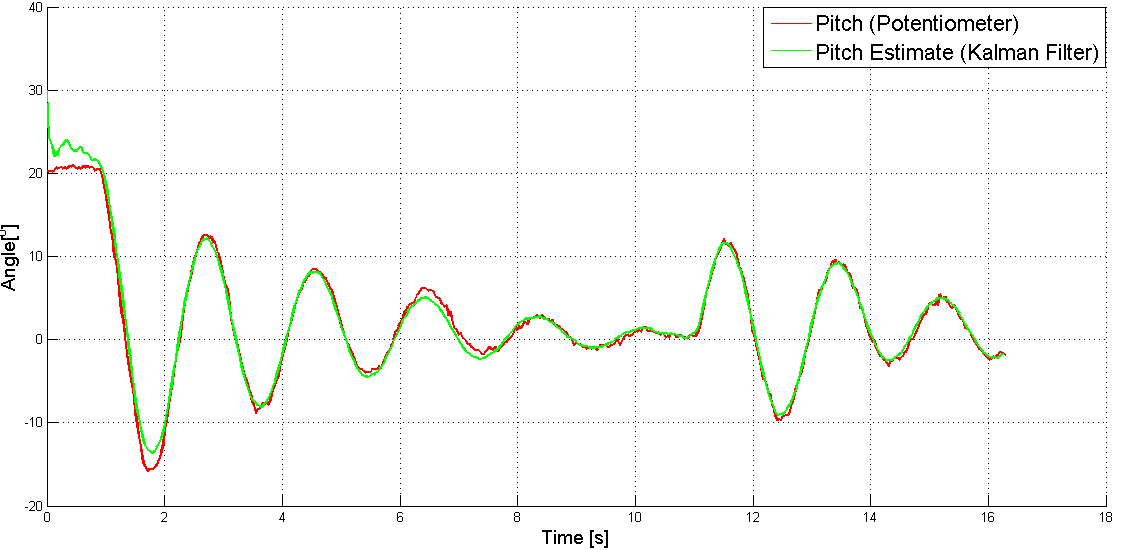
\includegraphics[width =0.8 \paperwidth]{\DocRoot/images/Kalman_low}
	\caption{Time-domain response of the Extended Kalman Filter}
	\label{Fig:Cross-Correlation of estimated pitch error1}
\end{figure}





\begin{comment}
\begin{figure}[h]
\renewcommand{\baselinestretch}{1.5} 	
\centering
\resizebox{14cm}{8cm}{\begin{tikzpicture}[auto, thick, node distance=2cm, >=triangle 45]

%
% Styles for states, and state edges
%
\tikzstyle{state} = [{rectangle, rounded corners, draw=black, very thick, text width=20.0em, minimum height=4em, text centered}]
\tikzstyle{stateEdgePortion} = [black,thick];
\tikzstyle{stateEdge} = [stateEdgePortion,->];
\tikzstyle{edgeLabel} = [pos=0.5, text centered, font={\sffamily\small}];


%
% Position States
%
\node[state, name=predict] {{{\LARGE}{\bf Model Update} (\enquote{Predict})}   \\ 
{   (1) Predict State  \\  \vspace{-0.25cm}
\hh $\hat{x}^{*}_{k} = \gls{Transitionmatrix}\hat{x}_{k-1} + \gls{Bmatrix}u_{k}$\\ 
(2) Predict Error Covariance \\ \vspace{-0.25cm}
\hh $\gls{covariancematrix}^* = \gls{Transitionmatrix}\gls{covariancematrix}_{-1}\gls{Transitionmatrix}^{\intercal} + \gls{noisecoplantmatrix}$}};


\node[state, name=correct, right of=predict, xshift=20em] {{\bf Measurement Update} (\enquote{Correct}) \\ 
{   (1) Compute Kalman Gain\\  \vspace{-0.25cm}
\hh $\gls{kalmangain}_{k} = \gls{covariancematrix}^*\gls{Cmatrix}^{\intercal}(\gls{Cmatrix}\gls{covariancematrix}^*\gls{Cmatrix}^{\intercal} + \gls{noisecomatrix})^{-1}$\\ 
(2) Update Estimate with Measurement $\gls{measurement}$ \\ \vspace{-0.25cm}
\hh $\hat{x}_k = \hat{x}^{*}_k + \gls{kalmangain}_k(z_k - \gls{Cmatrix}\hat{x}_k^{*})$\\
(3) Update Error Covariance  \\ \vspace{-0.25cm}
\hh $\gls{covariancematrix} = (I - \gls{kalmangain}_k\gls{Cmatrix})\gls{covariancematrix}^{*}$

}};


%
% Connect States via edges
%
\draw (predict.north) 
edge[stateEdge, bend left=45] node[edgeLabel, xshift=-3em]{} 
(correct.north); 

\draw ($(predict.west) + (0,2.5em)$) 
edge[stateEdgePortion] node[edgeLabel, yshift=+2.1cm]{} 
($(predict.east) + (0,2.5em)$); 

\draw (correct.south) 
edge[stateEdge, bend left=45] node[edgeLabel, xshift=-3em]{} 
(predict.south); 

\draw ($(correct.west) + (0,4.0em)$) 
edge[stateEdgePortion] node[edgeLabel, yshift=+2.1cm]{} 
($(correct.east) + (0,4.0em)$); 



% 
% inital states to start the filter
%
\node[ name=inital, below of=predict, left of=predict, xshift = -0.68em ,yshift=-8em]{Initial Estimates for $\hat{x}_{k-1}$ and $\gls{covariancematrix}_{-1}$};

\draw ($(inital.north) + (0,0)$) 
edge[stateEdge] node[edgeLabel, yshift=+2.1cm]{} 
($(predict.south) + (-5.4em,0)$); 
\end{tikzpicture}}
\caption{Kalman Filter flow diagram}
\label{fig:Kalman Filter flow diagram}
\end{figure}























\subsection{Block Diagram of the Kalman filter}
\pgfmathsetmacro{\lowergroup}{-8}
\pgfmathsetmacro{\lowerlowergroup}{-9.5}
\pgfmathsetmacro{\lqr}{-5.5}
\pgfmathsetmacro{\joint}{-6.5}
\pgfmathsetmacro{\cd}{-4.0}
\pgfmathsetmacro{\k}{-5.0}
\pgfmathsetmacro{\endpoint}{10}
\pgfmathsetmacro{\endpointtwo}{12}
\pgfmathsetmacro{\endpointthree}{14}
\pgfmathsetmacro{\noise}{1.5}
\begin{figure}[h]	
	\centering
	\begin{tikzpicture}[auto, thick, node distance=2cm, >=triangle 45]
	\draw
	% Drawing the blocks of first filter :
	node at (-0.3,0)     {$R$} 
	node at (5,2.3)     {\text{\footnotesize   Zero Mean Process Noise}} 
	node at (\endpointtwo+2,2.3)     {\text{\footnotesize  Zero Mean Measurement Noise}} 
	node at (3.2,\noise)      {\gls{noiseinsysystem}}
	node at (\endpointthree,\noise)      {\gls{noiseinoutput}}
	
	node at (0,0)      [input,name=input1,thick,above]{} 
	node at (3.5,\noise)      [input,name=noisesys,thick,above]{}
	node at (\endpointthree-.3,\noise)     [input,name=noisemea,thick,above]{}
	
	node at (1,0)              [sum={}{+}{-}{}]  (sum1) {}
	node at (6,0)              [sum={+}{+}{+}{}] (sum2) {}
	node at (\endpointtwo,0)             [sum={+}{+}{}{}]  (sum3) {}
	node at (\endpoint,\lowergroup)   [sum={}{+}{}{+}]  (sum4) {}
	node at (\endpointthree,\cd)           [sum={+}{-}{}{}]  (sum5) {}
	node at (\endpointthree,\joint)        [sum={+}{+}{}{}]  (sum6) {}
	
	node at (8,0) [block,scale=0.8](delay) {$q^{-1}$}
	node at (6,\lowergroup) [block,scale=0.8](delay2) {$q^{-1}$}
	node at (\endpointtwo,\lowergroup) [block,scale=0.8](delay3) {$q^{-1}$}
	
	node at (1,\cd) [gain,rotate=90,scale=0.6](lqr){SVF}
	
	node at (8,-2) [gain,scale=0.8,rotate=180](ad){$\gls{Transitionmatrix}$}
	node at (4.5,0)  [gain,scale=0.7](bd){$\gls{Bmatrix}_d$}
	node at (8,\lowergroup) [gain,scale=0.7](bd2){$\gls{Bmatrix}_d$}
	node at (10,0) [gain,scale=0.7](cd){$\gls{Cmatrix}_d$}
	node at (\endpointtwo,\cd) [gain,scale=0.7](cd2){$\gls{Cmatrix}_d$}
	node at (\endpointthree,\k)  [gain,scale=0.7,rotate=-90](k){$\gls{kalmangain}$}
	
	node at (\endpointthree-1,\noise) [gain,scale=1,rotate=180](couple){}
	node at (\endpointthree-1,\noise) {$\gls{couplingmatrixoutput}$}
	node at (4.5,\noise)  [gain,scale=0.8](gamma){$\gls{couplingmatrix}$}
	
	node at (2.5,0) [joint] (joint1) {}
	node at (9,0)   [joint] (joint2) {}
	% node at (\endpointthree,0)  [joint] (joint3) {}
	node at (\endpoint,\joint) [joint] (joint4) {}
	node at (\endpointthree,\lowergroup) [joint] (joint5) {};
	% Commands \draw with options like [->] must be written individually
	
	%	\draw(joint2) -- ++(0,-1.5) [->] -| node {} (sum1);
	\draw [->](input1)    -- node {} (sum1);
	\draw [->](sum1)      -- node {} (bd);
	\draw [->](bd)        -- node {} (sum2);
	\draw [->](sum2)      -- node {} (delay);
	\draw [->](delay)     -- node {} (cd);
	\draw [->](cd)        -- node {} (sum3);
	\draw [->](noisesys)  -- node {} (gamma);
	\draw [->](gamma)     -| node {} (sum2);
	\draw [->](noisemea)  -- node {} (couple);
	\draw [->](couple)    -| node {} (sum3);
	\draw [->](joint2)    |- node {} (ad);
	\draw [->](ad)        -| node {} (sum2);
	\draw [->](joint1)    |- node {} (delay2);
	\draw [->](delay2)    -- node {} (bd2);
	\draw [->](bd2)       -- node {} (sum4);
	\draw [->](delay3)    -- node {} (sum4);
	\draw [->](sum4)      |- node {} (cd2);
	\draw [->](cd2)       -- node {} (sum5);
	
	\draw [->](joint4)    -- node {} (sum6);
	\draw     (sum6)      -- node {} (joint5);
	\draw [->](joint5)    -- node {} (delay3);
	\draw [->](lqr)       -- node {} (sum1);
	\draw [->](k)         -- node {} (sum6);
	\draw [->](sum5)      -- node {} (k);
	\draw(joint5) --(\endpointthree,\lowerlowergroup) [->] -| node {} (lqr);
	
	\draw (sum3) --(\endpointthree,0) [->] -| node {} (sum5);		   
	% \draw [->](joint3)    -- node {} (sum5);		   
	%\draw    (sum3)      -- node {} (joint3);
	
	
	% Boxing and labelling noise shapers
	\draw [thick,dashed](3,2.8) rectangle (11,-2.7);
	\node at (2.8,3) [above=2mm, right=0mm] {\textsc{Plant}};
	\draw [thick,dashed](5,\cd+ 1.0) rectangle (\endpointthree+1,\lowerlowergroup-0.5);
	\node at (4.9,\cd + 0.8) [below=2mm, right=0mm] {\textsc{Observer}};
	\end{tikzpicture}
	\caption{Block diagram of the Kalman Filter}
	\label{fig: Kalman modely}
\end{figure}

\end{comment}
